\documentclass{article}
\usepackage{pgfplots}
\pgfplotsset{compat=1.18}

\begin{document}
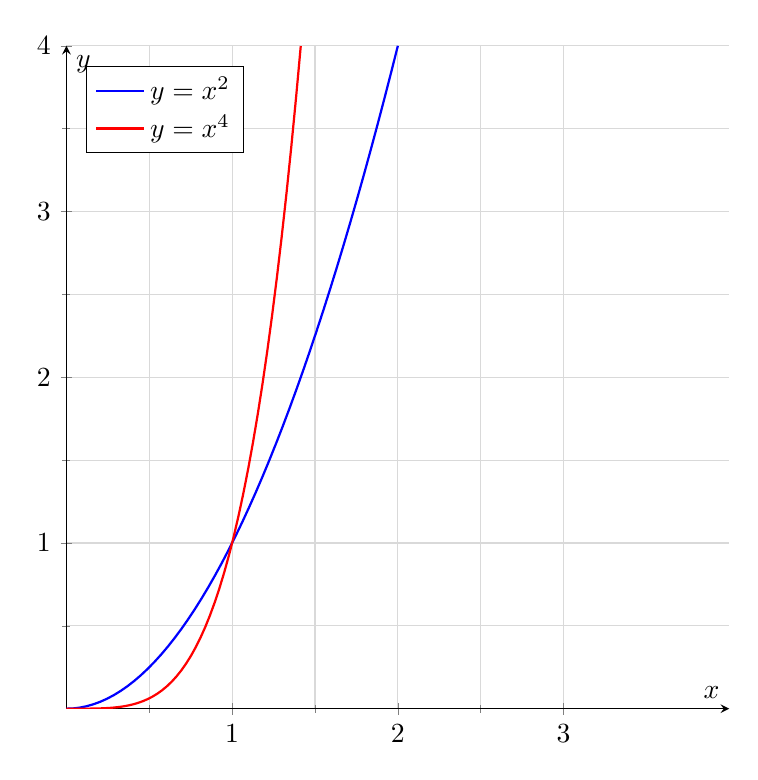
\begin{tikzpicture}
\begin{axis}[
    xlabel={$x$},
    ylabel={$y$},
    xmin=0, xmax=4,
    ymin=0, ymax=4,
    axis lines=middle,
    %xtick={0,0.5,1,1.5,2,2.5,3,3.5,4},   % x轴刻度
    xtick={0,1,2,3},   % x轴刻度
    ytick={0,1,2,3,4},
    minor tick num=1,                      % 每个主刻度之间一个小刻度（即0.1细度？此处为示范）
    grid=both,                             % 显示网格
    grid style={gray!30},
    width=10cm,
    height=10cm,
    legend pos=north west,
]
% 绘制 y = x^2, x从0到2
\addplot[domain=0:2, samples=50, thick, blue] {x^2};
\addlegendentry{$y=x^2$}
% 绘制 y = x^2, x从0到2
\addplot[domain=0:2^0.5, samples=50, thick, red] {x^4};
\addlegendentry{$y=x^4$}
\end{axis}
\end{tikzpicture}
\end{document}